\documentclass[10pt]{beamer}

\usepackage{tikz}
\usetikzlibrary{shadows}

\usepackage{beamerthemesplit}
\usepackage{amscd}
\usepackage{mathrsfs}
\usepackage{graphicx}
\usepackage{helvet}
%\usepackage[usenames]{color}

%%%=== beamer themes ===%%%

%%%  Check cheese online at:
%%%  https://www.hartwork.org/beamer-theme-matrix/

%\usetheme{berlin}
\usetheme{Szeged}

%\usecolortheme{beaver}
%\usecolortheme{rose}
%\usecolortheme{lily}
%\usecolortheme{beetle}
%\usecolortheme{crane}
\usecolortheme{seagull}
%\usecolortheme{wolverine}

\usefonttheme{professionalfonts}
%\usefonttheme{serif}
%\usefonttheme{structureitalicserif}
%
%\useinnertheme{rounded}
%\useinnertheme{inmargin}
%\useinnertheme{circles}
%
\useoutertheme{miniframes}
\useoutertheme{smoothbars}

%%%=== end of beamer themes ===%%%

%%%=== definitions ===%%%

\newcommand\mc{\mathscr}
\newcommand\mb{\mathbf}
\newcommand\inverse{\langle-1\rangle}
\newcommand\mathboxdot{\mathop{\boxdot}\limits}
\newcommand\mathodot{\mathop{\odot}\limits}
\newcommand\mathboxtimes{\mathop{\boxtimes}\limits}
\newcommand{\aatop}[2]{\genfrac{}{}{0pt}{}{#1}{#2}}

\newcommand\expcompk[1]{\mc{E}_k \langle{#1}\rangle}
\newcommand\expcomp[1]{\mc{E} \langle{#1}\rangle}

\DeclareMathOperator{\fix}{fix} \DeclareMathOperator{\aut}{aut}
\DeclareMathOperator{\lcm}{lcm} \DeclareMathOperator{\id}{id}
\DeclareMathOperator{\c.t.}{ct}\DeclareMathOperator{\Rec}{Rec}
\DeclareMathOperator{\Par}{Par}\DeclareMathOperator{\Fix}{Fix}

%%%=== end of definitions ===%%%

    \title[Data Science]{Data Science in Action}
    \author[vieplivee@gmail.com]{Ji Li}
    \institute[Yesware]{Data Scientist}
    \date{March 25, 2015}

\begin{document}

    \frame[plain]{\titlepage}

    \AtBeginSection[]
    {
     \begin{frame}
       \frametitle{Outline}
       \tableofcontents[currentsection]
     \end{frame}
    }

\section{What is Data Science}

  \subsection{Overview}

    \begin{frame}{Data science on Google search}
      \begin{center}
        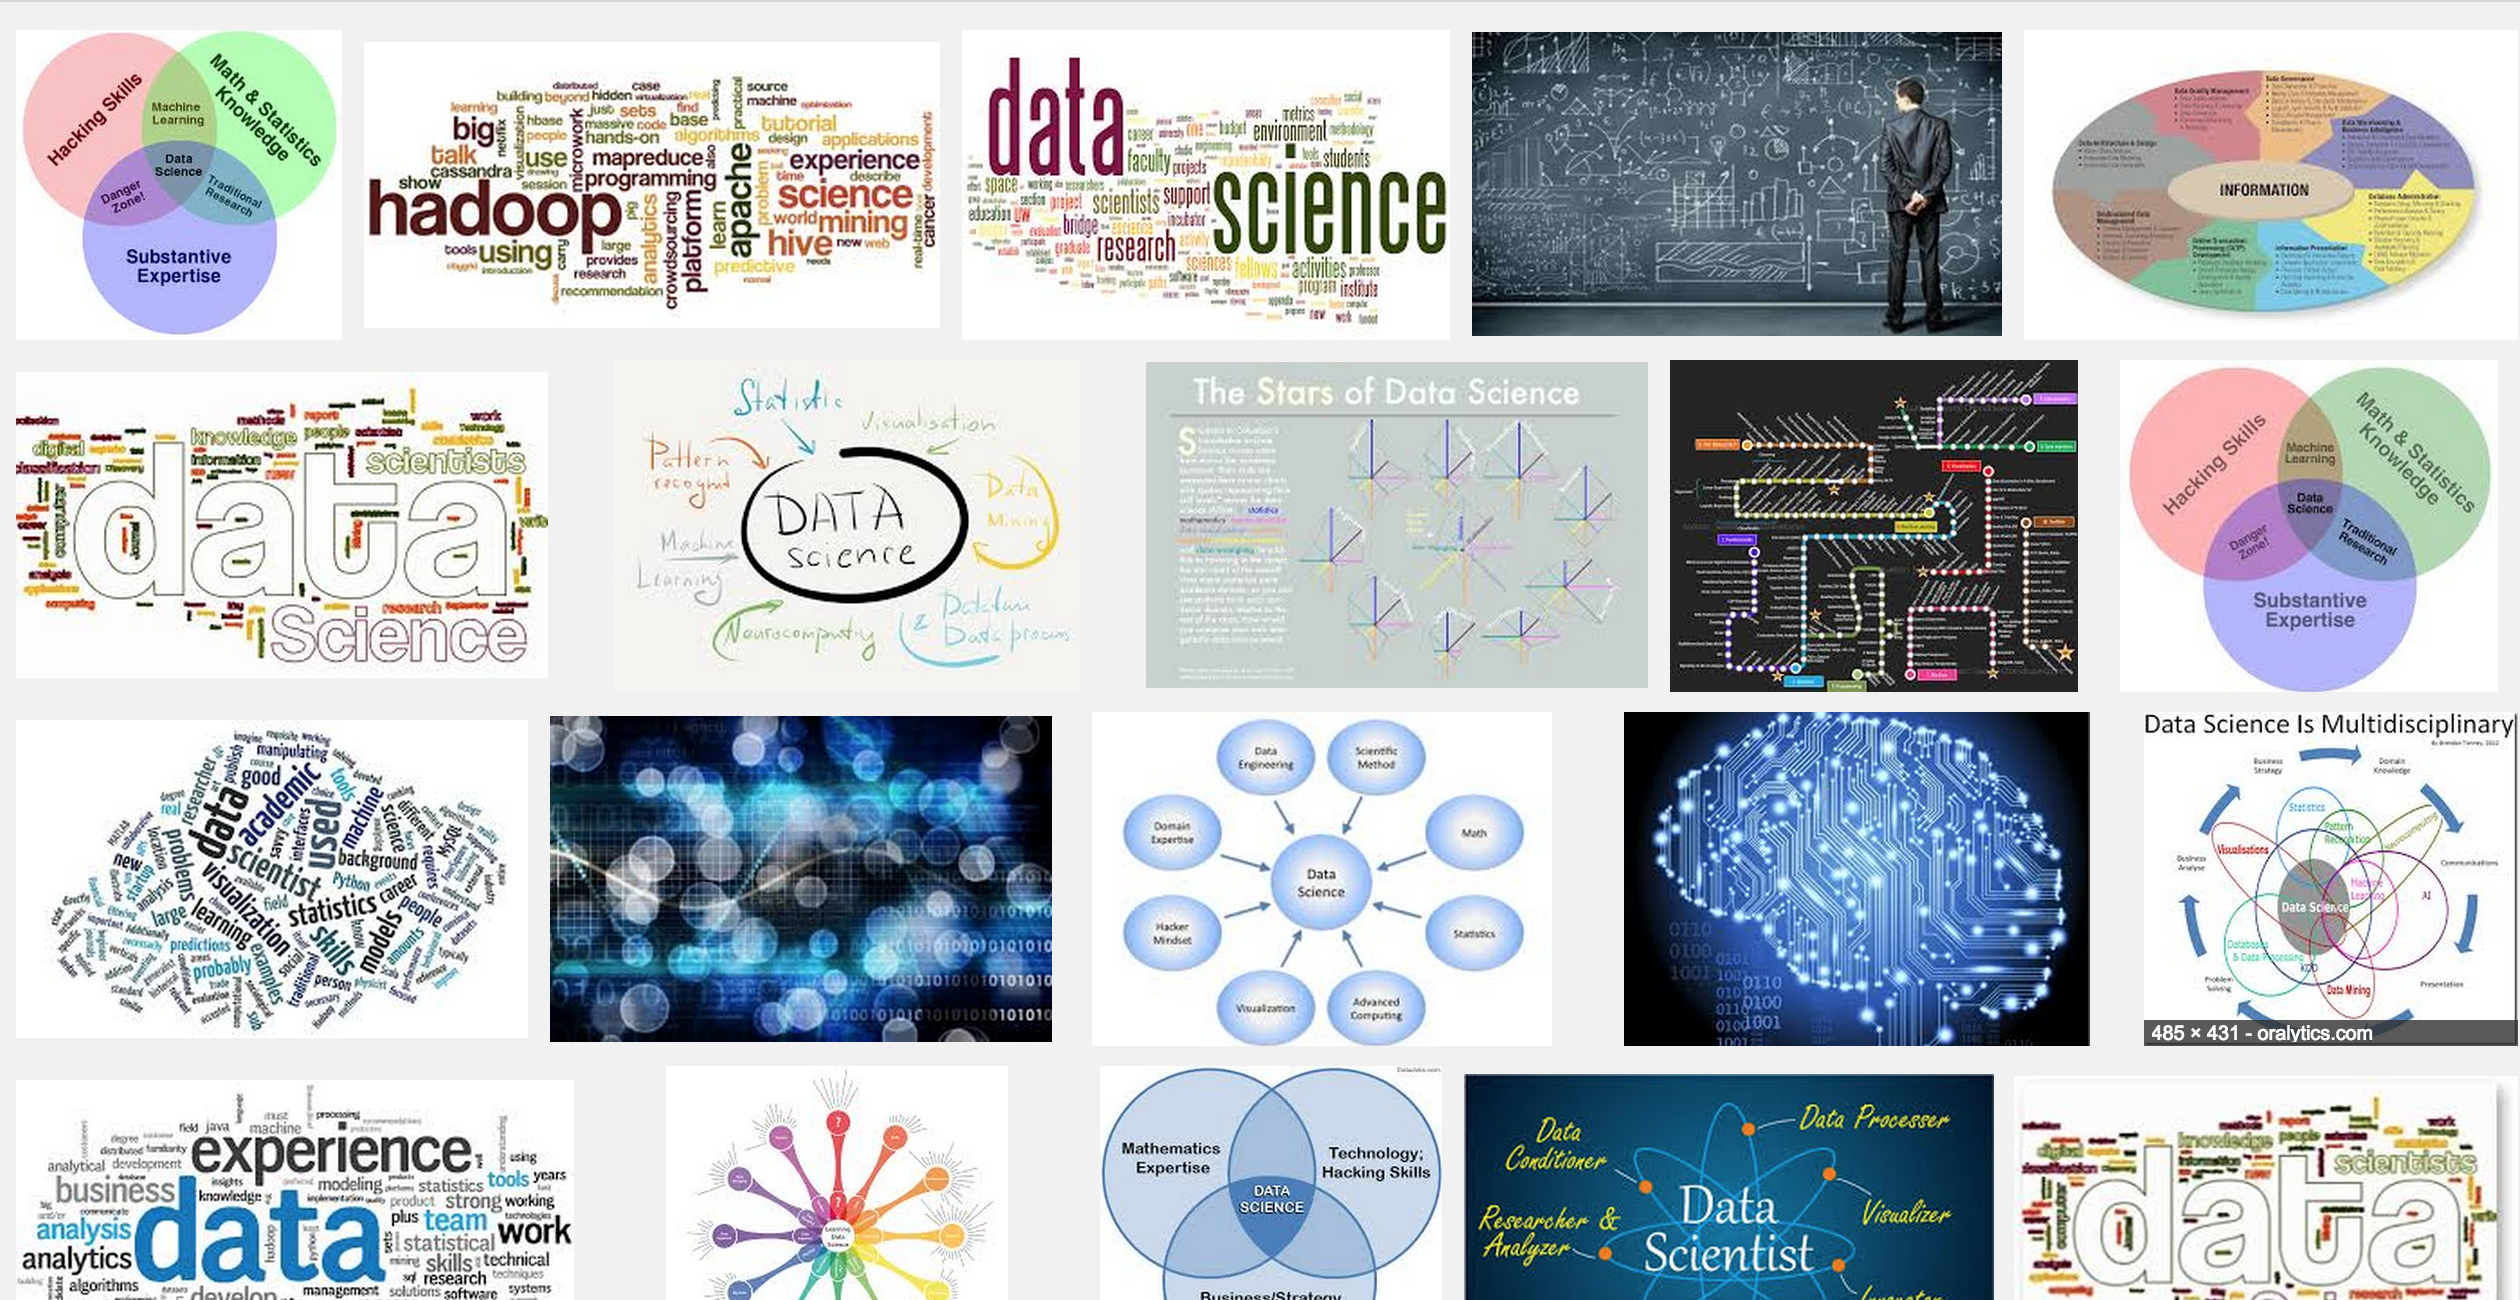
\includegraphics[width=300pt]{graphs/data_science_serach_result}
      \end{center}
    \end{frame}

    \begin{frame}{Data science from my point of view}
      \begin{center}
        \includegraphics[width=300pt]{graphs/data_science_structure}
      \end{center}
    \end{frame}

      \note{
        \begin{itemize}
        \item This is the version of data science I know.
        \item It by no means represent the general view point of the public.
        \end{itemize}
      }

  \subsection{Skills and Domain Expertise}
  
    \begin{frame}{Skills of a data scientist}
      \begin{center}
        \includegraphics[width=300pt]{graphs/data_science_skills}
      \end{center}
    \end{frame}

      \note{
        \begin{itemize}
        \item As a data scientist, you need to have SOME programming skills. For example, you'd need to find the right tools to work on the data in the way you want to, it being Python, R, or other means.
        \end{itemize}
      }

    \begin{frame}{Domain expertise of a data scientist}
      \begin{center}
        \includegraphics[width=300pt]{graphs/data_science_domain}
      \end{center}
    \end{frame}

    \begin{frame}{Doing data science}
      \begin{center}
        \includegraphics[width=300pt]{graphs/data_science_skills_domain}
      \end{center}
    \end{frame}

  \subsection{Python and R}

    \begin{frame}{Python and R for data science}
      \begin{center}
        \includegraphics[width=250pt]{graphs/python_r}
      \end{center}
      {\footnotesize
        iPython \url{http://goo.gl/zT4uPE}
        --- 
        RStudio \url{http://www.rstudio.com/}
      }
    \end{frame}

    % \begin{frame}{Python}
    %   \setbeamercovered{transparent}
    %   \begin{block}{Why Python}
    %     \begin{itemize}
    %       \pause \item The ``language of choice'' for data scientists.
    %       \pause \item Powerful packages: Numpy, Scipy, Scikit-Learn, Pandas.
    %       \pause \item Python is general purpose.
    %     \end{itemize}
    %   \end{block}
    %   \pause
    %   \begin{block}{Using Python}
    %     \begin{itemize}
    %       \pause \item iPython \url{http://goo.gl/zT4uPE}
    %       \pause \item Use Python for data munging.
    %       \pause \item Use Python for data mining.
    %       \pause \item Use Python for machine learning.
    %       \pause \item Use Python for data visualization.
    %     \end{itemize}
    %   \end{block}
    % \end{frame}

    % \begin{frame}{R}

    %   \begin{block}{Why R}
    %     \begin{itemize}
    %       \pause \item Strong support from the statistics community.
    %       \pause \item Powerful packages: ggplot2, dplyr, reshape2, etc.
    %     \end{itemize}
    %   \end{block}
    %   \pause
    %   \begin{block}{Using R}
    %     \begin{itemize}
    %       \pause \item RStudio \url{http://www.rstudio.com/}.
    %       \pause \item Use R for data munging.
    %       \pause \item Use R for data mining.
    %       \pause \item Use R for machine learning.
    %       \pause \item Use R for data visualization.
    %     \end{itemize}
    %   \end{block}
    % \end{frame}

\section{Data Science in Action}

    \subsection{Demo: Customer Churn Model}

      \begin{frame}{The quest}
        \setbeamercovered{transparent}
        \begin{block}{Definition of a churned customer}
        \end{block}
        \pause
        \begin{block}{Goal}
            \begin{itemize}
              \item Can we predict which customers will churn?
              \item What actions can we take to prevent the customers from churning?
            \end{itemize}
        \end{block}
        \pause
        \begin{block}{Data sets}
          \begin{itemize}
            \item Customer renew data.
            \item Customer support data.
            \item Customer account and demographic data.
            \item Customer usage data.
          \end{itemize}
        \end{block}
      \end{frame}

    \begin{frame}{First data set: customer renew data}
      \begin{center}
        \includegraphics[height=150pt]{graphs/dataset_customer_renew}
      \end{center}
    \end{frame}
    
    \begin{frame}{First data set: customer renew data - renewal schedule}
      \begin{center}
        \includegraphics[width=250pt]{graphs/dataset_renewal_schedule}
      \end{center}
    \end{frame}

    \begin{frame}{Second data set: customer support}
      \begin{center}
        \includegraphics[height=150pt]{graphs/dataset_customer_renew}
      \end{center}
    \end{frame}

    \begin{frame}{Third data set: customer account and demographic}
      \begin{center}
        \includegraphics[height=120pt]{graphs/dataset_customer_account}
      \end{center}
    \end{frame}

    \begin{frame}{Fourth data set: customer usage data}
      \begin{center}
        \includegraphics[height=110pt]{graphs/dataset_customer_usage}
      \end{center}
    \end{frame}

    \begin{frame}{Churn data structure}
      \begin{center}
        \includegraphics[height=180pt]{graphs/dataset_churn_str}
      \end{center}
    \end{frame}


    \subsection{(Optional) Demo: Predict Purchases after Trial}

\section{Some Afterwords}

  \subsection{Data Scientist Toolbox}

    \begin{frame}{Academia versus industry}
      \begin{center}
        \includegraphics[width=300pt]{graphs/academia_industry}
      \end{center}
    \end{frame}

    \begin{frame}{Data manipulation tools}
      \begin{center}
         \includegraphics[width=250pt]{graphs/data_tools}
      \end{center}
    \end{frame}

    \begin{frame}{Data visualization tools}
      \begin{center}
         \includegraphics[width=250pt]{graphs/data_visualization_tools}
      \end{center}
    \end{frame}
  
  \subsection{Data Science Books}

    \begin{frame}{Some books I enjoyed reading}
      \begin{itemize}
        \item Semiology of Graphics, http://goo.gl/Wh9YbkJacques Bertin, \url{http://goo.gl/Rl9XVm}
        \item The Grammar of Graphics, Leland Wilkinson, \url{http://goo.gl/ylYzUk}
        \item Applied Predictive Modeling, Max Kuhn, Kjell Johnson,http://goo.gl/n1pczx \url{http://goo.gl/Wh9Ybk}
        \item The Guru's Guide to Transact-SQL, Ken Henderson, \url{http://goo.gl/n1pczx}
      \end{itemize}
    \end{frame}
  
  \subsection{Daily Life of a Data Scientist}

    \begin{frame}{Sexy job?}    
      \begin{center}
         \includegraphics[width=300pt]{graphs/sexy_job}
      \end{center}
      {\footnotesize \url{https://hbr.org/2012/10/data-scientist-the-sexiest-job-of-the-21st-century/}}
    \end{frame}
    
    \begin{frame}{A typical day}
        \begin{columns}[T] % align columns
            \begin{column}{.48\textwidth}
                \color{blue}\rule{\linewidth}{4pt}
                We think...
                \begin{itemize}
                    \item Examine data
                    \item Run machine learning
                    \item Evaluate models using ROC
                    \item Create model report
                \end{itemize}                        
            \end{column}
        \hfill%
            \begin{column}{.48\textwidth}
                \color{red}\rule{\linewidth}{4pt}
                In real...
                \begin{itemize}
                    \item Munge data
                    \item Munge data
                    \item Munge data
                    \item Munge data
                \end{itemize}
            \end{column}
        \end{columns}
    \end{frame}
    
    \begin{frame}{Reality check: clustering}
        \begin{center}
        \includegraphics[width=280pt]{graphs/clustering_reality}
        \end{center}
    \end{frame}

    \begin{frame}{Thank You}
      \centerline{\large Email me: \texttt{vieplivee@gmail.com}}
    \end{frame}


\end{document}
